%%%%%%%%%%%%%%%%%%%%%%%%%%%%%%%%%%%%%%%%%%%%%%%%%%%%%%%%%%%%%%%%%%%%%%%%

%%% LaTeX Template for ECAI Papers 
%%% Prepared by Ulle Endriss (version 1.0 of 2023-12-10)

%%% To be used with the ECAI class file ecai.cls.
%%% You also will need a bibliography file (such as mybibfile.bib).

%%%%%%%%%%%%%%%%%%%%%%%%%%%%%%%%%%%%%%%%%%%%%%%%%%%%%%%%%%%%%%%%%%%%%%%%

%%% Start your document with the \documentclass{} command.
%%% Use the first variant for the camera-ready paper.
%%% Use the second variant for submission (for double-blind reviewing).

\documentclass{ecai} 

%\documentclass[doubleblind]{ecai} 

%%%%%%%%%%%%%%%%%%%%%%%%%%%%%%%%%%%%%%%%%%%%%%%%%%%%%%%%%%%%%%%%%%%%%%%%

%%% Load any packages you require here. 

\usepackage{latexsym}
\usepackage{amssymb}
\usepackage{amsmath}
\usepackage{amsthm}
\usepackage{booktabs}
\usepackage{enumitem}
\usepackage{graphicx}
\usepackage{color}

\usepackage[T1]{fontenc}
\usepackage{graphicx}
%\usepackage{color}
%\renewcommand\UrlFont{\color{blue}\rmfamily}

\usepackage{amsmath,amssymb,amsfonts}
% \usepackage[inline, shortlabels]{enumitem}
\usepackage{tabularx}
\usepackage{caption}
% \usepackage{titlesec}
\usepackage[english]{babel}
\captionsetup{font=it}
\usepackage{ragged2e}
\usepackage{hyperref}
\usepackage{pifont}
\usepackage{footmisc}
\usepackage{multirow}
\usepackage{algorithm2e}

% --- Tickz
\usepackage{physics}
\usepackage{amsmath}
\usepackage{tikz}
\usepackage{mathdots}
\usepackage{yhmath}
\usepackage{cancel}
\usepackage{color}
\usepackage{siunitx}
\usepackage{array}
\usepackage{multirow}
\usepackage{amssymb}
\usepackage{gensymb}
\usepackage{tabularx}
\usepackage{extarrows}
\usepackage{booktabs}
\usetikzlibrary{fadings}
\usetikzlibrary{patterns}
\usetikzlibrary{shadows.blur}
\usetikzlibrary{shapes}

% ---------

\usepackage{pdfpages}
\usepackage{booktabs}
\usepackage{csquotes}
\usepackage{lipsum}  
\usepackage{arydshln}
\usepackage{smartdiagram}
\usepackage[inkscapeformat=png]{svg}
\usepackage{textcomp}
\usepackage{tabularray}\UseTblrLibrary{varwidth}
\usepackage{xcolor}
\def\BibTeX{{\rm B\kern-.05em{\sc i\kern-.025em b}\kern-.08em
    T\kern-.1667em\lower.7ex\hbox{E}\kern-.125emX}}
% \usepackage{cite}
\usepackage{amsmath}
\newcommand{\probP}{\text{I\kern-0.15em P}}
\usepackage{etoolbox}

%%%%%%%%%%%%%%%%%%%%%%%%%%%%%%%%%%%%%%%%%%%%%%%%%%%%%%%%%%%%%%%%%%%%%%%%

%%% Define any theorem-like environments you require here.

\newtheorem{theorem}{Theorem}
\newtheorem{lemma}[theorem]{Lemma}
\newtheorem{corollary}[theorem]{Corollary}
\newtheorem{proposition}[theorem]{Proposition}
\newtheorem{fact}[theorem]{Fact}
\newtheorem{definition}{Definition}

%%%%%%%%%%%%%%%%%%%%%%%%%%%%%%%%%%%%%%%%%%%%%%%%%%%%%%%%%%%%%%%%%%%%%%%%

%%% Define any new commands you require here.

% \newcommand{\BibTeX}{B\kern-.05em{\sc i\kern-.025em b}\kern-.08em\TeX}

\renewcommand{\arraystretch}{1.7}

\setlength{\extrarowheight}{2.5pt}
\renewcommand{\arraystretch}{0.2}
\renewcommand{\arraystretch}{1.7}

\newcommand{\before}[1]{\textcolor{red}{#1}}
\newcommand{\after}[1]{\textcolor{green}{#1}}

\newcommand{\old}[1]{\textcolor{orange}{#1}}
\newcommand{\rem}[1]{\textcolor{red}{#1}}
\newcommand{\todo}[1]{\textcolor{orange}{\newline \textit{\textbf{TODO:} #1}} \newline \newline }



\newcounter{relation}
\setcounter{relation}{0}
\renewcommand{\therelation}{\arabic{relation}}
\newcommand{\relationautorefname}{Relation}

\newenvironment{relation}[1][]{%
    \refstepcounter{relation}%
    \noindent \raggedright \textit{\textbf{Relation. \therelation}} \hfill$}
{%
$ \hfill \phantom{x}

}

\newcounter{proof}
\setcounter{proof}{0}
\renewcommand{\theproof}{\arabic{proof}}
\newcommand{\proofautorefname}{Proof}

\renewenvironment{proof}[1][]{
    \refstepcounter{proof}
    \noindent \raggedright \textit{\textbf{Proof. \theproof}}

    \setlength{\leftskip}{1em}

}
{

\
\setlength{\leftskip}{0pt}
}

%%%%%%%%%%%%%%%%%%%%%%%%%%%%%%%%%%%%%%%%%%%%%%%%%%%%%%%%%%%%%%%%%%%%%%%%

\begin{document}

%%%%%%%%%%%%%%%%%%%%%%%%%%%%%%%%%%%%%%%%%%%%%%%%%%%%%%%%%%%%%%%%%%%%%%%%

\begin{frontmatter}

    %%% Use this command to specify your submission number.
    %%% In doubleblind mode, it will be printed on the first page.

    \paperid{123}

    %%% Use this command to specify the title of your paper.

    \title{Unveiling Cooperative Intelligence: Towards Explainable Multi-Agent Reinforcement Learning with Organizational Models}

    % JS: keywords:
    %     Multi-Agent Reinforcement Learning
    %     Explainability
    %     Organizational Models
    %     Cooperative Intelligence

    %%% Use this combinations of commands to specify all authors of your 
    %%% paper. Use \fnms{} and \snm{} to indicate everyone's first names 
    %%% and surname. This will help the publisher with indexing the 
    %%% proceedings. Please use a reasonable approximation in case your 
    %%% name does not neatly split into "first names" and "surname".
    %%% Specifying your ORCID digital identifier is optional. 
    %%% Use the \thanks{} command to indicate one or more corresponding 
    %%% authors and their email address(es). If so desired, you can specify
    %%% author contributions using the \footnote{} command.

    \author[A,B]{\fnms{Julien}~\snm{Soulé}\thanks{Corresponding Author. Email: julien.soule@lcis.grenoble-inp.fr}}
    \author[A]{\fnms{Jean-Paul}~\snm{Jamont}}
    \author[A]{\fnms{Michel}~\snm{Occello}}
    \author[B]{\fnms{Louis-Marie}~\snm{Traonouez}}
    \author[C]{\fnms{Paul}~\snm{Théron}}

    \address[A]{Univ. Grenoble Alpes, Grenoble INP, LCIS, 26000, Valence, France}
    \address[B]{Thales Land and Air Systems, BL IAS, Rennes, France}
    \address[C]{AICA IWG, La Guillermie, France}

    %%% Use this environment to include an abstract of your paper.

    \begin{abstract}
        This paper addresses the challenge of explainability in Multi-Agent Reinforcement Learning (MARL) by proposing a novel algorithm leveraging the $\mathcal{M}OISE^+$ Organizational Model. While previous studies have focused on understanding individual agent behaviors in traditional RL, our work emphasizes the need to elucidate the implicit cooperation among multiple agents in MARL systems. We introduce the \emph{Partial Relation between Agents' History and Organizational Model} (PRAHOM) algorithm, which links agents' histories to organizational specifications, facilitating the inference of cooperative structures from trained agents' behaviors. PRAHOM serves dual purposes: constraining the learning process based on organizational constraints and inferring organizational specifications from trained agents' histories. PRAHOM is designed to constrain agent policy spaces and generate valuable organizational specifications. Empirical evaluations conducted in cooperative Atari-like game environments validate the effectiveness of our algorithm, showing alignment with hand-crafted expectations and superior performance in some scenarios. This work seeks to contribute to AI explainability in MARL systems by offering a principled framework for understanding emergent cooperative behaviors. By bridging the gap between individual agent decision-making and cooperation, our algorithm aims to enhance transparency and interpretability in complex Multi-Agent Systems.
    \end{abstract}

\end{frontmatter}

%%%%%%%%%%%%%%%%%%%%%%%%%%%%%%%%%%%%%%%%%%%%%%%%%%%%%%%%%%%%%%%%%%%%%%%%

\section{Introduction}

% Context
Explainable Artificial Intelligence (XAI) has emerged as a critical requirement for the widespread adoption of AI systems, particularly in multi-agent settings where multiple agents interact and cooperate to achieve complex goals~\citep{doshivelez2017rigorous,gunning2019xai}. While significant progress has been made in explaining the behavior of single agents~\citep{ribeiro2016classifier,lundberg2017unified}, the challenge of explicating the cooperative strategies and emergent organizational structures in Multi-Agent Reinforcement Learning~\citep{busoniu2008survey} (MARL) systems is not largely addressed~\citep{kok2006collaborative,omidshafiei2019learning}.

% Problem
In MARL systems, a set of trained agents can achieve goals through implicit cooperation and coordination. However, very few works have attempted to analyze the trained agents' policies to make this cooperation explicit and attempt to handle it directly~\citep{albrecht2018survey,perolat2017pool}. This lack of explainability hinders: \quad i) the understanding of the complex social, cooperation, and coordination schemes that emerge between the trained agents in a bottom-up manner; \quad ii) the application of these schemes to agents to guide their training in a top-down manner, hence providing safety guarantees.
Addressing these concerns would improve the trust and adoption of MARL systems in real-world applications~\citep{kok2006collaborative,omidshafiei2019learning}.

% The idea of benefitting of the particularly adaptive and general MARL mechanism to get an approximated suited MAS organization and producing associated specifications, requires to link the MARL training of a set of policies in a bidirectional way with a MAS organizational model. For instance, a hierarchy described in a MAS model would constrain the possible policies to get ultimately trained in MARL. Reversely, a set of trained policies could be described in an organizational model, thus indicating resemblance with known MAS organization architectures.

% Contribution
To address this problem, we propose a novel algorithm called PRAHOM that leverages the $\mathcal{M}OISE^+$ organizational model~\citep{hubner2007moise} as a common ground to provide explicating the cooperative aspects in the observed agents' behaviors, or making these agents' policies constrained regarding expected cooperative schemes. The underlying idea is to establish a relationship between the agents' histories and the organizational specifications, such as roles, goals, or social links.

The characterization of organizational aspects uses predefined relations to identify matching histories as organizational specifications. Otherwise it proposes a first approach relying on a series of statistical and unsupervised learning techniques to automatically infer new unnamed organizational specifications, hence enriching known organizational specifications and their relations with agents' histories.
The constraining of policies regarding organizational constraints associated to agents, leverages on relations to know expected histories in order to constrain agents to choose foreseen actions when required so they stick to the expected behaviors.

% This paper first informally introduce the aforementioned broad idea as a new specific research study we refer to as \textquote{Organizational Multi-Agent Reinforcement Learning} (OMARL). We present DMO (Dec-POMDP $\mathcal{M}OISE^+$ OMARL) a first attempt to formally describe OMARL processes using the Decentralized Partially Observable Markov Decision Process (Dec-POMDP) as model for MARL and $\mathcal{M}OISE^+$ as an organizational model. Then, we propose PRAHOM (Partial Relations between Agents' Histories and Organizational Model), a DMO process that allows both getting some organizational specifications from \textquote{trained} policies and constraining policies training with respect to given specifications. As PRAHOM only changes the action set and relies \textquote{observed} actions, it is agnostic of the MARL algorithm used jointly with function approximators as policies. We used PRAHOM within a proposed design approach to generate an efficient organization and associated OCPV specifications based on the environment, the initial design constraints, and goals.

% Results
We showed that PRAHOM effectively constrains the resulting agents' policy space according to the specified organizational constraints. Additionally, we demonstrate that PRAHOM can produce valuable organizational specifications from trained agents' histories. The PRAHOM algorithm is evaluated in cooperative Atari-like game environments, where the inferred organizational specifications generally match or outperform the expected hand-crafted expected results.

% Outline
The remainder of the paper is organized as follows: Section 2 provides theoretical background on MARL and organizational modeling. Section 3 introduces the PRAHOM algorithm and its formal foundations. Section 4 describes the experimental setup and evaluation environments. Section 5 presents and discusses the results of our empirical evaluation. Section 6 reviews related work, and Section 7 concludes the paper and outlines future research directions.

%%%%%%%%%%%%%%%%%%%%%%%%%%%%%%%%%%%%%%%%%%%%%%%%%%%%%%%%%%%%%%%%%%%%%%%%

% JS : A GARDER SI ON EN A BESOIN

% \begin{eqnarray}\label{eq:vcg}
% p_i(\boldsymbol{\hat{v}}) & = &
% \sum_{j \neq i} \hat{v}_j(f(\boldsymbol{\hat{v}}_{-i})) - 
% \sum_{j \neq i} \hat{v}_j(f(\boldsymbol{\hat{v}})) 
% \end{eqnarray}

% \begin{theorem}[Fermat, 1637]\label{thm:fermat}
% No triple $(a,b,c)$ of natural numbers satisfies the equation 
% $a^n + b^n = c^n$ for any natural number $n > 2$.
% \end{theorem}

% \begin{proof}
% A full proof can be found in the supplementary material.
% \end{proof}

% \begin{table}[h]
% \caption{Locations of selected conference editions.}
% \centering
% \begin{tabular}{ll@{\hspace{8mm}}ll} 
% \toprule
% AISB-1980 & Amsterdam & ECAI-1990 & Stockholm \\
% ECAI-2000 & Berlin & ECAI-2010 & Lisbon \\
% ECAI-2020 & \multicolumn{3}{l}{Santiago de Compostela (online)} \\
% \bottomrule
% \end{tabular}
% \end{table}

%%%%%%%%%%%%%%%%%%%%%%%%%%%%%%%%%%%%%%%%%%%%%%%%%%%%%%%%%%%%%%%%%%%%%%%%

\section{Related works and positioning}

% présenter une revue "complète" de la littérature connexe dans les domaines de l'apprentissage par renforcement multi-agents (MARL) et de l'IA explicable.

% discuter des algos précédents pour améliorer l'explicabilité dans les systèmes MARL et identifier les lacunes dans la recherche existante.

MARL is a machine learning paradigm where agents learn to make decisions by interacting with an environment. The goal is for a set of agents to maximize the cumulative reward over time through a process of trial and error.
MARL makes it possible to automatically converge towards policies enabling the given objective to be achieved. Reinterpreting these individual policies into organizational specifications requires work on explainability at a collective level that is rarely addressed in the literature.

\paragraph{\textbf{Framework for MARL with organizational aspects}}
%
Some proposed frameworks attempt to include organizational concepts within the MARL framework.
Kazhdan and. al.~\cite{Kazhdan2020} present a library to improve the explainability of MARL systems by bringing them closer to symbolic models, in particular to infer roles.%todo
%
Wang et. al.~\cite{Wang2020} introduce an approach in which similar emerging roles are pushed to jointly specialize on specific tasks.
%
Tosic et. al~\cite{Tosic2010} proposes a framework for coordination based on the communication capabilities of multi-agent systems.
%
Zheng et. al.~\cite{Zheng2018} presented a platform for MARL that aims to facilitate research on artificial collective intelligence by providing a comprehensive set of evaluation metrics to compare the performance of MARL algorithms.

\paragraph{\textbf{Characterization of emerging collective strategies}}
%
Heuillet and. al.~\cite{Heuillet2022} propose an approach to explain cooperative strategies using Shapley values. Its effectiveness has been demonstrated in the context of applications on multi-agent particle environments by explaining certain decisions taken.
%
Jaques and. al.~\cite{Jaques2019} propose a mechanism to benefit from communication between agents by rewarding agents having a causal influence on other agents. This approach leads to learned communication protocols allowing for overall more efficient collective behavior.

\paragraph{\textbf{Adaptation of MARL to meet requirements}}
%
Shao et. al.~\cite{Shao2022} introduces an approach based on the leader-follower model as a mechanism to improve multi-agent cooperative tasks with dynamic characteristics, aiming to improve the adaptability and generalization of MARL systems.
%
Roy and. al.~\cite{Roy2020} presents two policy regularization methods aimed at improving coordination in reinforcement learning.
% %
\emph{Specification-Guided Reinforcement Learning} aims to generate policies that accomplish a specific task using external specifications to guide learning in achieving an objective and under given constraints~\cite{Bansal2022}.% ~\cite
%
~Jothimurugan et. al.~\cite{Jothimurugan2021} propose logical specification learning as exploiting the compositional structure of specifications to generate policies for complex tasks.

\

To our knowledge, there is no work that can be used to generate organizational specifications for an MAS achieving a given objective in an environment and respecting possible additional organizational constraints.
Unlike these works, our originality is to explicitly use an organizational model as a general means of expressing policies at a collective level and/or constraining their learning with respect to requirements.

\section{Theoretical foundations}

% introduire les fondements théoriques de notre algo:
%   - apprentissage par renforcement multi-agents (MARL)
%   - cadre du modèle organisationnel des systèmes multi-agents (MOISE+) et montrer sa pertinence pour améliorer l'explicabilité de l'IA au sein du MARL.

% détailler l'algorithme PRAHOM en décrivant ses composants et fonctionnalités...

% fournir des preuves formelles de son efficacité dans la restriction des espaces de politiques des agents durant et après l'apprentissage par rapport à des spécifications organisationnelles considérées comme des contraintes.

% fournir des preuves (formelles dans l'idéal) de son efficacité dans la génération de spécifications organisationnelles à partir des historiques des agents entrainés.

In this section, we first introduce the basics PRAHOM is relying on concerning MARL and the $\mathcal{M}OISE^{+}$ organizational model. Then, we formally describe how agents' policies and training process within MARL can be linked to the $\mathcal{M}OISE^{+}$ organizational model.

\subsection{MARL model}

The chosen MARL model is based on the Decentralized Partially Observable Markov Decision Process (Dec-POMDP)~\citep{Oliehoek2016} because it considers multiple agents in a similar MAS fashion. It relies on stochastic processes to model uncertainty of the environment for the changes induced by actions, in received observations, in communication\dots Additionally, unlike Partially Observable Stochastic Games (POSG), the reward function can be common to agents which fosters training for collaborative oriented actions~\citep{Beynier2013}.
A Dec-POMDP $d \in D$ (with $D$ the set of Dec-POMDP) is a 7-tuple $d = (S,\{A_i\},T,R,\{\Omega_i\},O,\gamma)$ , where:
\begin{itemize}
    \item $S = \{s_1, ..s_{|S|}\}$: The set of the possible states.
    \item $A_{i} = \{a_{1}^{i},..,a_{|A_{i}|}^{i}\}$: The set of the possible actions for agent $i$.
    \item $T$ so that $T(s,a,s') = \probP{(s'|s,a)}$ : The set of conditional transition probabilities between states
    \item $R: S \times A \times S \rightarrow \mathbb{R}$: The reward function
    \item $\Omega_{i} = \{o_{1}^{i},..,o_{|\Omega_{i}|}^{i}\}$: The set of observations for agent $ag_i$
    \item $O$ so that $O(s',a,o) = \probP{(o|s',a)}$ : The set of conditional observation probabilities.
    \item $\gamma \in [0,1]$, the discount factor
\end{itemize}

Considering $m$ \textbf{teams} (also referred as \textbf{groups}) each containing several agents among $\mathcal{A}$, we also detail the minimal formalism notation we re-used for solving the Dec-POMDP for a given team $i, 0 \leq i \leq m$ containing $n$ agents~\citep{Beynier2013,Albrecht2024}:

\begin{itemize}

    \item $\Pi$: the set of policies. A \textbf{policy} $\pi \in \Pi, \pi: \Omega \rightarrow A$ deterministically maps an observation to an action. It represents the agent's internal logic;
    \item $\Pi_{joint}$: the set of joint-policies. A \textbf{joint-policy} $\pi_{joint} \in \Pi_{joint}, \pi_{joint}: \Omega^n \rightarrow A^n = \Pi^n$ chooses an action for each agent regarding their respective observation. It can be viewed as a set of the policies used in agents;
    \item $H$: the set of histories. A \textbf{history} over $z \in \mathbb{N}$ steps (where $z$ is generally the maximum number of steps for an episode) is the $z$-tuple $h = ((\omega_{k}, a_{k}) | k \leq z, \omega \in \Omega, a \in A)$
    \item $H_{joint}$: the set of joint-histories. A \textbf{joint-history} over $z \in \mathbb{N}$ steps $h_{joint} \in H_{joint}, h_{joint} = \{h_1,h_2..h_n\}$ is the set of the agents' histories.
    \item $U_{joint,i}(<\pi_{joint,i}, \pi_{joint,-i}>): \Pi_{joint} \rightarrow \mathbb{R}$: gives the \textbf{expected cumulative reward} over a finite horizon (if $\gamma < 1$ or the number of steps in an episode is finite), with $\pi_{joint,i}$ the joint policy for team $i$ and $\pi_{joint,-i}$ all of the other concatenated joint-policies (considered as fixed);
    \item $BR_{joint,i}(\pi_{joint,i}) = argmax_{\pi_{joint,i}}(U(<\pi_{joint,i},\pi_{joint,-i}>))$: gives the \textbf{best response} $\pi_{joint,i}^*$ in the sense that the team cannot change any of the policies in the joint-policy $\pi_{joint,i}^*$ to get a better expected cumulative reward than $U_i^* = U_{joint,i}(<\pi_{joint,i}^*, \pi_{joint,-i}>)$;
    \item $SR_{joint,i}(\pi_{joint,i}, s) = \{\pi_{joint,i} | U(<\pi_{joint,i},\pi_{joint,-i}>) \geq s\}$: gives the \textbf{sufficient response} as the set of joint-policies getting at least $s \in \mathbb{R}, s \leq U_i^*$ as expected cumulative reward.
\end{itemize}

We refer to \textbf{solving} the Dec-POMDP for the team $i$ as finding a joint policy $\pi_{joint,i} \in \Pi_{joint}, \pi_{joint,i} = BR_{joint,i}(\pi_{joint,i})$ that maximize the expected cumulative reward over a finite horizon.
We refer to \textbf{sub-optimally solving} the Dec-POMDP at $s$ expectancy as finding a the joint policies $\pi_{joint,i} \in \Pi_{joint}, \pi_{joint,i} = SR_{joint,i}(\pi_{joint,i}, s)$ that gets the expected cumulative reward over a finite horizon at least at $s \in \mathbb{R}, s \leq U_i^*$.


\subsection{Organizational model}

Among, the existing organizational models \textquote{Agent/Group/Role}~\citep{Ferber2004} and $\mathcal{M}OISE^+$~\citep{Hubner2002} provide a relevant high-level description of the structures and interactions within the MAS. However, we favor $\mathcal{M}OISE^+$ because it provides an advanced formal description for an organization without incompatibilities with MARL, especially for formal description of agents' policies. It takes into account explicitly the social aspects between agents where \textquote{AGR} focuses on the integration of standards oriented towards design. Additionally, it provides a sufficiently detailed vision of organization to be understood at different point of views.
Based on $\mathcal{M}OISE^+$~\citep{Hubner2007} formalism, we only give the minimal elements of the formalism we used.

\paragraph{\textbf{Organization specifications (OS)}}: $\mathcal{OS} = \langle \mathcal{SS}, \mathcal{FS}, \mathcal{DS} \rangle$, the set of all organization specifications, where $\mathcal{SS}$ are the \textbf{Structural Specifications}, $\mathcal{FS}$ are the \textbf{Functional Specifications}, and $\mathcal{DS}$ are the \textbf{Deontic Specifications}

\paragraph{\textbf{Structural Specifications (SS)}}: $\mathcal{SS} = \langle \mathcal{R}, \mathcal{IR}, \mathcal{G} \rangle$, where:

\begin{itemize}

    \item $\mathcal{R}_{ss}$: the set of all roles (denoted $\rho \in \mathcal{R}$);

    \item $\mathcal{IR}: \mathcal{R} \rightarrow \mathcal{R}$: the inheritance relation between roles ($\mathcal{IR}(\rho_1) = \rho_2$ means $\rho_1$ inherits from $\rho_2$ also denoted $\rho_1 \sqsubset \rho_2$);

    \item $RG \subseteq GR$ the set of root groups, $GR = \langle \mathcal{R}, \mathcal{SG}, \mathcal{L}^{intra}, \mathcal{L}^{inter}, \mathcal{C}^{intra}, \mathcal{C}^{inter}, np, ng \rangle$, the set of all groups, where

          \begin{itemize}

              \item $\mathcal{R} \subseteq \mathcal{R}_{ss}$: the set of non-abstract roles;

              \item $\mathcal{SG} \subseteq \mathcal{GR}$: the set of sub-groups;

              \item $\mathcal{L} = \mathcal{R} \cross \mathcal{R} \cross \mathcal{TL}$: the set of links. A link is a 3-tuple $(\rho_s,\rho_d,t) \in \mathcal{L}$ (also denoted as a predicate $link(\rho_s,\rho_d,t))$, where $\rho_{s}$ is the source role, $\rho_{d}$ is the destination role, and $t \in \mathcal{TL}, \mathcal{TL} = \{acq, com, aut\}$ is the link type;
                    \begin{itemize}
                        \item If $t = acq$ (acquaintance), the agents playing the source role $\rho_{\mathrm{s}}$ are allowed to have a representation of the agents playing the destination role $\rho_{d}$;
                        \item If $t = com$ (communication), the $\rho_{\mathrm{s}}$ agents are allowed to communicate with $\rho_{d}$ agents;
                        \item If $t = aut$ (authority), the $\rho_{\mathrm{s}}$ agents are allowed to have authority on $\rho_{d}$ agents. It requires an acquaintance and communication link.
                    \end{itemize}
              \item $\mathcal{L}^{intra} \subseteq \mathcal{L}$: the set of intra-group links;
              \item $\mathcal{L}^{inter} \subseteq \mathcal{L}$: the set of inter-group links;

              \item $\mathcal{C} = \mathcal{R} \cross \mathcal{R}$: the set of compatibilities. A compatibility is a couple $(a,b) \in \mathcal{C}$ (also denoted $\rho_a \bowtie \rho_b$), means agents playing role $\rho_a \in \mathcal{R}$ can also play role $\rho_b \in \mathcal{R}$;
              \item $\mathcal{C}^{intra} \subseteq \mathcal{C}$: the set of intra-group compatibilities;
              \item $\mathcal{C}^{inter} \subseteq \mathcal{C}$: the set of inter-group compatibilities;

              \item $np: \mathcal{R} \rightarrow \mathbb{N} \times \mathbb{N}$: the relation giving the cardinality of agents adopting a role;
              \item $ng: \mathcal{SG} \rightarrow \mathbb{N} \times \mathbb{N}$: the relation giving the cardinality of each sub-group.

          \end{itemize}

\end{itemize}

\paragraph{\textbf{Functional Specifications (FS)}}: $\mathcal{FS} = \langle \mathcal{SCH}, \mathcal{PO} \rangle$, where:

\begin{itemize}
    \item $\mathcal{SCH} = \langle\mathcal{G}, \mathcal{M}, \mathcal{P}, mo, nm \rangle$: the set of \textbf{social scheme}, where:
          \begin{itemize}
              \item $\mathcal{G}$ is the set of global goal;

              \item $\mathcal{M}$ is the set of mission labels;
              \item $\mathcal{P} = \langle \mathcal{G}, \{\mathcal{G}\}^s, OP, [0,1] \rangle, s \in \mathbb{N}^*$ is the set of plans that builds the tree structure of the goals.
                    %
                    A plan $p \in \mathcal{P}$ is 4-tuple $p=(g_f,\{g_i\}_{0 \leq i \leq s}, op, ps), g_f \in \mathcal{G}, g_i \in \mathcal{G}, op \in OP, OP = \{sequence, choice, parallel\}, ps \in [0,1]$, meaning that the goal $g_f$ is achieved if some of the sub-goals $g_i$ are achieved with a success probability $ps$ and according to the operator $op$:
                    %
                    \begin{itemize}
                        \item if $op = sequence$, the $g_i$ can only be achieved in the same order sequentially;
                        \item if $op = choice$, only one of the $g_i$ has to be achieved;
                        \item if $op = parallel$, the $g_i$ can only be achieved sequentially or simultaneously.
                    \end{itemize}

              \item $mo: \mathcal{M} \rightarrow \mathbb{P}(\mathcal{G})$: specifies the set of goals a mission is associated to;
              \item $nm: \mathcal{M} \rightarrow \mathbb{N} \times \mathbb{N}$ the cardinality of agents committed for each mission.
          \end{itemize}
    \item $\mathcal{PO}: \mathcal{M} \cross \mathcal{M}$: the set of \textbf{preference order}. A preference order is couple $(m_1, m_2), m_1 \in \mathcal{M}, m_2 \in \mathcal{M}$ (also denoted $m_{1} \prec m_{2}$) meaning that if there is a moment when an agent is permitted to commit to $m_{1}$ and also $m_{2}$, it has a social preference for committing to $m_{1}$.
\end{itemize}

\paragraph{\textbf{Deontic Specifications (DS)}}: $\mathcal{DS} = \langle \mathcal{OBL},\mathcal{PER} \rangle$, the set of deontic specifications, where:

\begin{itemize}
    \item $\mathcal{TC}$: the set of \textbf{time constraints}. A time constraint $tc \in \mathcal{TC}$ specifies a set of periods during which a permission or obligation is valid ($Any \in \mathcal{TC}$ means everytime);
    \item $\mathcal{OBL}: \mathcal{R} \cross \mathcal{M} \cross \mathcal{TC}$: the set of \textbf{obligations}. An obligation is a 3-tuple $(\rho_a,m,tc)$ (aslo denoted $obl(\rho_a,m,tc)$) meaning an agent playing role $\rho_a \in \mathcal{R}$ is obliged to commit on mission $m \in \mathcal{M}$ for a given time constraint $tc \in \mathcal{TC}$;
    \item $\mathcal{PER}$: the set of \textbf{permissions}. A permission is a 3-tuple $(\rho_a,m,tc)$ (aslo denoted $per(\rho_a,m,tc)$) meaning an agent playing role $\rho_a \in \mathcal{R}$ is permitted to commit on mission $m \in \mathcal{M}$ for a given time constraint $tc \in \mathcal{TC}$;
\end{itemize}

\subsection{Linking MARL and Organizational model}

We refer to Organizational oriented MARL (OMARL) as all the processes linking MARL and Organization model as for being able to get information from joint-policies to build an organizational model, and constraining possible output joint-policies subset regarding organizational specifications. We refer to \emph{Dec-POMDP $\mathcal{M}OISE^+$ OMARL} (DMO) as all the formally described OMARL process using the Dec-POMDP for MARL and $\mathcal{M}OISE^+$ for the organizational model.

In a DMO process, we consider solving sub-optimally the Dec-POMDP $d \in D$ for a single team $i$ (comprising $n$ agents in $\mathcal{A}$) at a $s = U_i^* - \delta$ (with $\delta \in \mathbb{R}$) expectancy, we may obtain a set $S\Pi_{joint,i,s} = SR_{d,joint,i}(\pi_{joint,i},s) = \{\pi_{joint,i,s,1}, \pi_{joint,i,s,2} .. \pi_{joint,i,s,m}\}$ with the $\pi_{joint,i,s,k} \in \Pi_{joint}$ ($k \in \mathbb{N}, k \leq m$) and $SR_{d,joint,i}(\pi_{joint,i},s)$ gives the sub-optimal joint-policies at $s$ expectancy for the Dec-POMDP $d$ also denoted $SR_{joint,i,s}(d)$. For instance, we may have $m$ different convergent joint-policies reaching a given expected cumulative reward after several training due to non-deterministic parameters in training.

Yet as an extra constraint, we only want joint-policies allowed by the constraining organizational specifications $\mathcal{OS}_{cons}$ we denote $S\Pi_{joint,i,\mathcal{OS}_{cons}} = \{\pi_{joint,i,\mathcal{OS}_{cons},1}, \pi_{joint,i,\mathcal{OS}_{cons},2} .. \pi_{joint,i,\mathcal{OS}_{cons},b}\}$ with $b \in \mathbb{N}$ and the $\pi_{joint,i,\mathcal{OS}_{cons},k} \in \Pi_{joint}$ ($k \in \mathbb{N}, k \leq b$). Then, one can envision to use the sub-optimal joint-policies that satisfy the specifications $S\Pi_{joint,i,s} \cap S\Pi_{joint,i,\mathcal{OS}_{cons}}$, on which we can infer further associated specifications $\mathcal{OS}_{s,i}$ of the implicit resulting organization.

As a summary, a first general definition for a DMO process is a relation between the sub-optimal joint-policies set and associated organizational specifications set the following way:

\

\begin{relation}\label{rel:def_dmo}
    dmo: D \times \mathcal{OS}_{cons} \rightarrow (S\Pi_{joint,i,s} \cap S\Pi_{joint,i,\mathcal{OS}_{cons}}) \times \mathcal{OS}_{i,s}
\end{relation}
Can be understood as for a given problem comprising a environment and a goal to be achieved by agents, and some design constraints; we can possibly get sufficiently successful trained agents that are compliant with given specifications, and some associated organizational specifications.

In practice, implementing a DMO process faces two main issues:
%
\begin{enumerate}
    \item The intractability in analyzing policies directly because policy function approximations (such as neural networks) are generally difficult to explain hence hindering the extraction of organizational specifications;
    \item The lack of common ground between policies and organizational specifications enabling to know how agents are expected to behave when they are constrained to stick to organizational specifications. Reversly, there is no way to characterize any organizational specifications regarding behavior induced by agents' policies.
\end{enumerate}

To address (1), we hypothetize that for a single deterministic policy $\pi_q: \Omega_q \rightarrow A_q$ having been played over $l \in \mathbb{N}$ episodes hence $H_l = \{\langle (\omega_{j,k}, a_{j,k}), 0 \leq k \leq p_l, p_l \in \mathbb{N}, \omega_k \in \Omega_q, a_k \in A_q \rangle, 0 \leq j \leq l\}$, if there is $e \in \mathbb{N}$, $l \geq e$ and if many different observations $|\{\omega_{j,k}, 0 \leq j \leq l, 0 \leq k \leq p_l\}|$ are obtained, then the difference between the actual policy and the reconstructed policy $\pi_q^r: = {(\omega_{j,k}, a_{j,k}), 0 \leq j \leq l, 0 \leq k \leq p_l}$ is small $\delta_q^r = \pi_q \backslash \pi_q^r, |\delta_q^r| \leq b, 0 \leq b \leq |\pi_q|$.

In other words, we hypothetize we can approximate the apparent behavior of a deterministic policy by saving all of the observation-action couples we can observe as a set. Thus, instead of analyzing policies directly, we only take agents' histories (obtained by letting play policies) into account to analyse their behaviors.

Continuing the previous approach, we address (2) by introducing a relation $osh: \mathcal{OS} \rightarrow \mathcal{P}(H_{joint})$ theoretically linking any organizational specification to a subset of expected joint-histories (practically expressed in short way as patterns).
Using that relation, we proposed the \autoref{rel:def_extended_dmo} that we showed is indeed compliant to initial $dmo$ definition \autoref{rel:def_dmo} in \autoref{proof:to_extended_dmo}.

\begin{relation}\label{rel:def_extended_dmo}
    $\\$ dmo: D \times \mathcal{OS}_{cons} \rightarrow (SR_{joint,i,s}[D] \cap rct[osh[\mathcal{OS}_{cons}]]) \times osh^{-1}[obs[SR_{joint,i,s}[D]] \cap osh[\mathcal{OS}_{cons}]]
\end{relation}

\

\noindent With $rct: H_{joint} \rightarrow \Pi_{joint} = \{\pi = \{(\omega_i, a_i), 0 \leq i \leq z\}, h = \langle (\omega_i, a_i), 0 \leq i \leq z \rangle, h \in H_{joint}\}$. The relation to reconstruct a joint-policy from a joint-history.
\noindent With $obs: \Pi_{joint} \rightarrow H_{joint} = \{h = \langle (\omega_l, a_l) \in \pi \rangle, l \in \mathbb{N}, \pi = \{ (\omega_i, a_i), 0 \leq i \leq z \}, \pi \in \Pi_{joint}\}$. The relation to save a joint-history from a joint-policy.

\

\begin{proof}\label{proof:to_extended_dmo}

    Let $dmo: D \times \mathcal{OS}_{cons} \rightarrow (SR_{joint,i,s}[D] \cap rct[osh[\mathcal{OS}_{cons}]]) \times osh^{-1}[obs[SR_{joint,i,s}[D]] \cap osh[\mathcal{OS}_{cons}]]$ \\

    By definition, $(SR_{joint,i,s}[D] \cap rct[osh[\mathcal{OS}_{cons}]]) = (S\Pi_{joint,i,s} \cap S\Pi_{joint,i,\mathcal{OS}_{cons}})$ \\

    By definition, $osh^{-1}[obs[SR_{joint,i,s}[D]] \cap osh[\mathcal{OS}_{cons}]] = osh^{-1}[obs[\Pi_{joint,i,s}] \cap H_{joint,i,\mathcal{OS}_{cons}}] = osh^{-1}[H_{joint,i,s} \cap H_{joint,i,\mathcal{OS}_{cons}}]$

    With $H_{joint,i,s} \cap H_{joint,i,\mathcal{OS}_{cons}} = H_{joint,i,\mathcal{OS}_{cons}}^{'} \subseteq H_{joint,i,\mathcal{OS}_{cons}}$

    Hence, $osh^{-1}[H_{joint,i,\mathcal{OS}_{cons}}^{'}] = \mathcal{OS}_{cons}^{'} \subseteq \mathcal{OS}_{cons}$

    Finally, $dmo_{2}: D \times \mathcal{OS}_{cons} \rightarrow (S\Pi_{joint,i,s} \cap S\Pi_{joint,i,\mathcal{OS}_{cons}}) \times \mathcal{OS}_{i,cons}$

    Hence, $dmo_{2} \subseteq dmo$
\end{proof}

From \autoref{rel:def_extended_dmo}, except from regular MARL training we notice a DMO process intended contribution to be represented by:
\begin{enumerate}
    \item $rct[osh[\mathcal{OS}_{cons}]]$: highlighting the need to know the expected joint-histories for a given organizational specifications and how to use these joint-histories to constrain the joint-policies during training.
    \item $osh^{-1}[obs[SR_{joint,i,s}[D]] \cap osh[\mathcal{OS}_{cons}]]$: highlighting the need to sample (optionally constrained) joint-histories and to infer organizational specifications from them.
\end{enumerate}

Addressing the implementation of these intended contributions led to the development of the PRAHOM algorithm as a first attempt to implement a DMO process.

\subsection{Details of the PRAHOM algorithm}

Continuing the previous decomposition in two activities, we detailed our process to get the specifications out of the agents' policies; and the process to get the joint-policies satisfying given specifications. PRAHOM is then a synthesis of these two processes presented in \autoref{alg:PRAHOM}.

\RestyleAlgo{ruled}
\SetKwComment{Comment}{// }{}

\begin{algorithm}[hbt!]
    \caption{Partial Action-based $\mathcal{M}OISE^+$ Identification DMO (PRAHOM)}\label{alg:PRAHOM}

    \KwData{$d \in D$, the Dec-POMDP to solve}
    \KwData{$ep_{max} \in \mathbb{N}$, the maximum number of episodes}
    \KwData{$step_{max} \in \mathbb{N}$, the maximum number of steps per episodes}
    \KwData{$s \in \mathbb{R}$, the cumulative reward expectancy}
    \KwData{$\pi_{joint}$, the joint-policies to be trained}
    \KwData{$\mathcal{OS}_{cons} \in \mathcal{OS}_{cons}$, the design specifications to respect}
    \KwData{$Solv: \Pi \times A \times O \times \mathbb{R} \rightarrow \Pi$, the MARL algorithm for updating a single policy in order to solve the Dec-POMDP}

    \KwResult{$(s\pi_{joint,s,i} \in S\Pi_{joint,s,i}, os_{s,i} \in \mathcal{OS}_{s,i})$, the sub-optimal policies associated organization specifications}

    $s\pi_{joint,s,i} = PRAHOM-osh-training(s,i)$

    $os_{s,i} = PRAHOM-hos(s\pi_{joint,s,i})$

\end{algorithm}

\paragraph{\textbf{Infering OS from joint-policies}}

% Schéma général de PRAHOM-HOS (PRAHOM-History to Organizational Specification) :

% PRAHOM-HOS:
%
%  if h_i is (at least partially) known
%     apply KOSI (Knowledge-based Organizational Identification) approach
%
%  else apply GOSI (General Organizational Specification Infering) approach
%    1) SS:
%       1) infer roles & roles inheritance relations (via sequence clustering)
%       2) groups, (via analysis of agents social impact)
%       3) infer compatibilities (via comparison between analyzed joint histories)
%       4) infer intra & extra links (via analysis of roles social impact in a given group / all groups)
%       5) infer roles agents cardinality (via comparison between analyzed joint histories)
%       6) infer sub-groups cardinality (via comparison betwee analyzed joint-histories)
%
%    2) FS:
%       1) infer goals, plans (via threshold states analysis, generalized role behavior analysis...)
%       2) infer missions (unifying goals and associated agents and analysis of goal tree structure to determine goals shared by several agents)
%       3) infer mission to goals (via generalization over analyzed joint-histories)
%       4) infer agents' cardinality for each mission (via generalization over analyzed joint-histories)
%
%    3) DS
%       1) infer permissions & obligations (via generalization over analyzed joint-histories)

We propose some relations between $\mathcal{M}OISE^+$ specifications and joint-histories. Their premises comes from noticing some specifications in the $\mathcal{M}OISE^+$ organizational model can be obviously mapped to subsets of actions from a single sub-optimal joint-policy, we propose the following relations:

\begin{itemize}
    \item $rh: \mathcal{R} \rightarrow \mathcal{P}(H)$: gives the histories associated with a role
    \item $sgh: \mathcal{SG} \rightarrow \mathcal{P}(H)$: gives the histories associated with a subgroup
    \item $lh: \mathcal{L} \rightarrow \mathcal{P}(H)$: gives the histories associated with an intra link
    \item $gh: \mathcal{G} \rightarrow \mathcal{P}(H)$: gives the histories associated with a global goal
    \item $mh: \mathcal{M} \rightarrow \mathcal{P}(H)$: gives the histories associated with a mission label
\end{itemize}

From these relation, we propose to rely on the previous relations through \emph{PRAHOM-hos} presented in \autoref{alg:PRAHOM-hos} that is consistent with $pos$.

\RestyleAlgo{ruled}
\SetKwComment{Comment}{// }{}

\begin{algorithm}[hbt!]
    \caption{PRAHOM-hos}\label{alg:PRAHOM-hos}
    \KwData{$\pi_{joint}$, the joint-policies to be analyzed}
    \KwResult{$os \in OS$, the associated organization specifications}

    $h_{joint} = testEpisode(\pi_{joint})$

    \ForEach{$h_{joint,i} \in h_{joint}$}{
        \ForEach{$h_{j} \in h_{joint,i}$}{

            $r_j = \langle r, determineRoles(h_{j}) \rangle$

            $sg_j = determineSubgroups(h_{j})$

            $l_j = determineIntraLinks(h_{j})$

            $g_{ind,j} = determineIndGoals(h_{j})$

            $m_{ind,j} = determineIndMissions(h_{j})$

            $p_{ind,j} = determineIndPlans(h_{j}, m_{ind,j}, g_{ind,j})$

        }

        $g = determineGoals(g, h_{joint,i}, {g_{ind,j}})$

        $m = determineMissions(m, h_{joint,i}, {m_{ind,j}})$

        $p = determinePlans(p, h_{joint,i}, {p_{ind,j}})$

        $mo = determineMissionToGoals(mo, g_i, m_i)$
    }

    $ng = determineSgCard(\{r_j\}_i)$

    $np = determineRoleCard(\{r_j\}_i)$

    $c = determineIntraCompatibilities(\{r_j\}_i)$

    $per = determinePermissions(\{r_j\}_i, m)$

    $obl = determineObligations(\{r_j\}_i, m)$

    $nm = determineAgentCardPerMission(mo)$

    $ss = \langle \{r_j\}_i, \{sg_j\}_i, \{l_j\}_i, \emptyset, c, \emptyset, np, ng \rangle$

    $fs = \langle {g, m, p, mo, nm}, \emptyset \rangle$

    $ds = \langle per, obl \rangle$

    $os = \langle ss, fs, ds \rangle$

\end{algorithm}

As we have only one group, we do not consider the inter-links and inter-compatibilities. Additionally as a simplification, we consider only one social scheme. As a general remark, the \textquote{determine*} relations are not all fully described and rely on custom implementation.

PRAHOM-hos first look at the individual level.
First, it tries to figure out the roles played by agents ($determineRoles$) by sampling history sub-sequences $h \in H$ and comparing with known history sub-sequences whose we know the associated role via $ra$.
Then, it tries to get the intra links the agent has with other agents. ($determineIntraLinks$ and $determineInterLinks$) via $lh$.
Then, it tries to known the subgroup where the agent is ($determineSubgroup$) via $sgh$.
Then, it tries to know the individual goals the agent aim to ($determineIndGoals$) via $gh$.
Then, it tries to know the mission the agent is committed to ($determineIndMissions$) via $mh$.
Finally, it tries to build a part of the plan the agent is playing at its individual level ($determineIndPlans$) via $ph$ and the inferred individual goal and the inferred individual mission.

Then PRAHOM-hos look at the social and collective level.
At the end of each joint-policy we try to reinforce a global view of the goals $g$, missions $m$, plans $p$, and the knowledge of the mission to goal $mo$; with the partially inferred information at the individual level.

At the end of the algorithm, it tries to synthesize the knowledge infered until know to have better view of the number of agent per subgroup $ng$, the agent cardinality per mission $nm$, the role cardinality $np$, the compatibilities between roles $c$, the permissions and obligations $per$ and $obl$.


\paragraph{\textbf{Constraining joint-policies satisfying OS}}

\

We consider a given MARL algorithm that iteratively converges towards a joint-policy so that each agent's policy is updated at each step until a finite horizon. In \autoref{proof:jpc_to_ac} we proved that constraining the available action set for each agent to the action sets authorized by the organization specifications at each step of the MARL training; implies constraining the converged joint-policies to the ones that satisfy the given organization specifications. We used that result, to setup our $sop$ used jointly with MARL learning through \emph{PRAHOM-osh-training} presented in \autoref{alg:PRAHOM-osh-training}.

\RestyleAlgo{ruled}
\SetKwComment{Comment}{// }{}

\begin{algorithm}[hbt!]
    \caption{PRAHOM-osh-training}\label{alg:PRAHOM-osh-training}
    \KwData{$d \in D$, the Dec-POMDP to solve}
    \KwData{$ep_{max} \in \mathbb{N}$, the maximum number of episodes}
    \KwData{$step_{max} \in \mathbb{N}$, the maximum number of steps per episodes}
    \KwData{$s \in \mathbb{R}$, the cumulative reward expectancy}
    \KwData{$\pi_{joint}$, the joint-policies to be trained}
    \KwData{$\mathcal{OS}_{cons} \in \mathcal{OS}_{cons}$, the design specifications to respect}
    \KwData{$solv: \Pi \times A \times O \times \mathbb{R} \rightarrow \Pi$, the MARL algorithm for updating a single policy in order to solve the Dec-POMDP}
    \KwResult{$s\pi_{joint} \in S\Pi_{joint,s,i}$, the sub-optimal joint-policies that satisfy the design specifications}

    $forbidden = \Pi_{joint} \setminus (DMO-pos^{-1}(\mathcal{OS}_{cons}))$

    $s\pi_{joint} = \{\}$

    \ForEach{$1 \leq ep \leq ep_{max}$}{

        $h_{joint} = \{\emptyset^n\}$

        $\omega_{0} = \emptyset$

        $a_{0} = \emptyset$

        \ForEach{$1 \leq step \leq step_{max}$}{

            \ForEach{$\pi_i \in \pi_{joint}$}{

                $\omega_{step} = getObservation()$

                $r_{step} = getReward()$

                $\pi_{i,step} = Solv(\pi_{i,step-1}, \omega_{step-1}, a_{step-1}, r_{step})$  \Comment*[r]{Update the individual policy}

                $A_{step} = \{a | (\omega_{step}, a) \in \pi, \pi \in \pi_{joint},\pi_{joint} \notin forbidden, \{(\omega', a') \in h\} \in \pi\}$ \Comment*[r]{Restricted available actions}

                $a_{step} = \pi_{i,step}(\omega_{step})$ \Comment*[r]{Choose next action}

                $h_{joint,i} = \langle h_{joint,i}, (\omega_{step}, a_{step}) \rangle$ \Comment*[r]{Update the history}

            }

        }
    }

    $s\pi_{joint} = \{\pi_{joint}\}$


\end{algorithm}

\emph{PRAHOM-osh-training} first converts the $\mathcal{OS}_{cons} \in \mathcal{OS}_{cons}$ design specifications into a $forbidden$ set of the non-authorized joint-policies. It uses a non-described reverse \emph{PRAHOM-hos} algorithm to achieve it.

Then, \emph{PRAHOM-osh-training} uses a given MARL algorithm to update the agents' individual policies with previous action, observation and resulting reward. Then, it first computes the authorized actions set $A_{step}$ according to the current history $h_{joint,i}$. Then, an action is chosen among authorized actions. That action $a_{step}$ is added in history to be used for updating the agent's policy in the next step.
Finally, considering only one iteration of episode, it returns a sub-optimal joint-policy $\pi_{joint}$ satisfying $\mathcal{OS}_{cons}$
We can note the $\mathcal{OS}_{cons}$ could forbid the MARL algorithm to provide a joint-policy that reaches a expected cumulative reward.


\section{Methodology}

% décrire la méthodologie pour évaluer PRAHOM
%   - configuration expérimentale: les environnements de jeu coopératifs PettingZoo de type Atari avec les paramètres spécifiques utilisés, présentation et utilisation de "PRAHOM Wrapper" pour intégrer PRAHOM dans les environnements de jeu.
%   - mesures utilisées pour évaluer l'efficacité de notre algo et fournir un aperçu du processus de collecte et d'analyse des données.

In order to assess PRAHOM, we considered using \emph{PRAHOM} in available simulated environments made up of agents that have to achieve a goal with the best performance through various collective strategies whose some can be easily understood.
We selected three Atari-like environments for their visual rendering is a convenient way to assess the results with manual observations\footnotemark[1].
We also considered a Cyberdefense environment as a first attempt to apply \emph{PRAHOM} in a non-visual Cyberdefense environment:

\footnotetext[1]{Additional explanation and the examples discussed using \emph{PRAHOM PettingZoo wrapper} are available at \url{https://github.com/julien6/omarl_experiments?tab=readme-ov-file\#tutorial-predator-prey-with-communication}}


\begin{itemize}
    \item \textquote{Drone swarm - 3rd CAGE Challenge}~\cite{cage_challenge_3_announcement} (CYB) consists of cyberdender agents deployed on networked drones fighting against maliciously deployed malware programs. We may expect agents to \allowbreak isolate compromised drones;
    \item \textquote{Pistonball} (PBL)~\cite{Terry2021} is a series of pistons to bring a ball from right to left side hence requiring neighbors' representation;
    \item \textquote{Predator-prey with communication}~\cite{Lowe2017} (PPY) consists of predators monitored by a leader to catch faster prey hence requiring hunting strategies;
    \item \textquote{Knights Archers Zombies}~\cite{Terry2021} (KAZ) consists in knights and archers learning how to kill zombies hence requiring efficient agent spatial positioning.
\end{itemize}
%
\noindent We applied PRAHOM in three cases:
\begin{itemize}
    \item No organizational specifications (NTS): agents have to learn an efficient collective strategies without any constraints or indications.
    \item Partially constraining organizational specifications (PTS): some constraints are given to help converge faster or meet requirements.
    \item Fully constraining organizational specifications (FTS): manually crafted joint-policies are given for they are a reference regarding learned joint-policies.
\end{itemize}

\noindent Here, we do not present the details of the constraints that were given in NTS and FTS (available in Git repository\footnotemark[1]).


\section{Results and discussion}

% présenter les résultats de nos évaluations empiriques
%   - performances de l'algorithme PRAHOM vis-à-vis des contraintes dans l'espaces des politiques des agents et la génération de spécifications organisationnelles à partir des historiques des agents entrainés

% discuter des implications de nos résultats et mettre en évidence toutes les observations ou tendances notables observées au cours des expériences.

% discussion complète des implications de nos résultats et de leur signification plus large dans le contexte de MARL et du XAI

% explorer les explications potentielles des résultats observés

% discuter des limites de notre algo et proposons des pistes de recherche future pour remédier à ces limites.

\begin{figure}[h!]
    \centering
    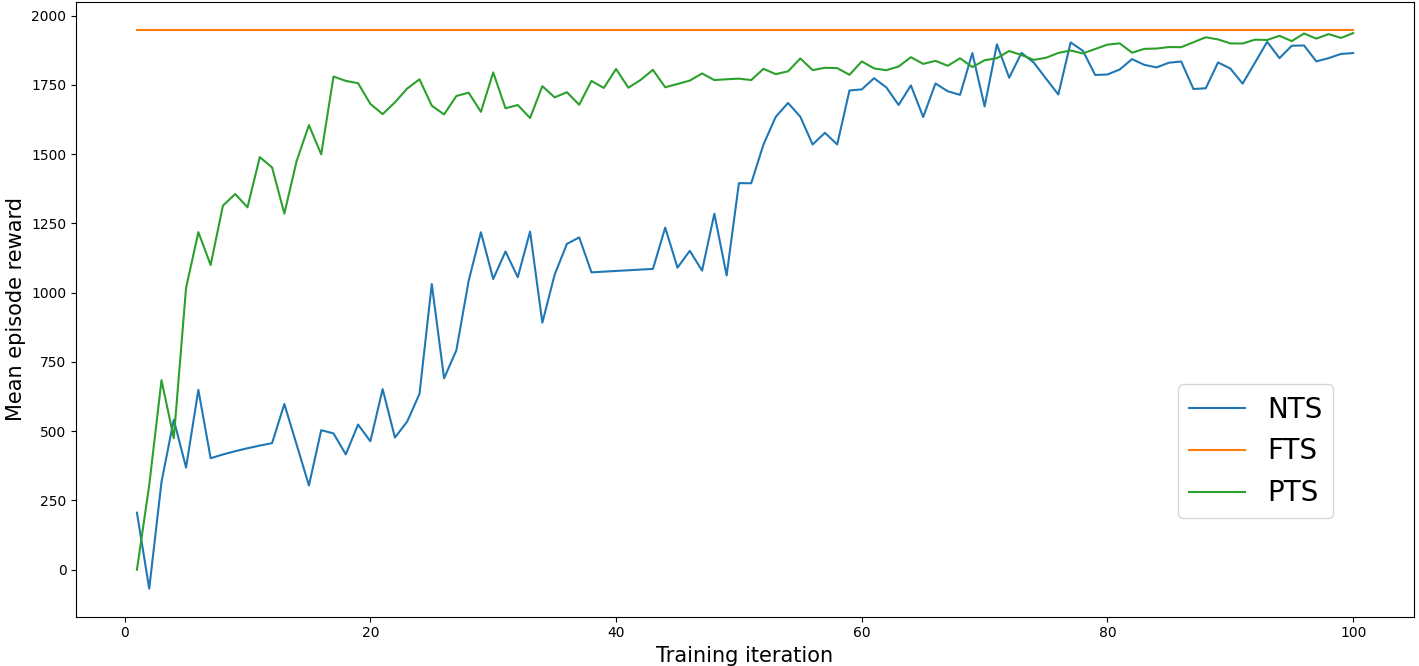
\includegraphics[width=0.46\textwidth]{figures/prahom_learning_curve.png}
    \caption{Average reward for each iteration in the PBL environment for the NTS, PTS, and FTS cases}
    \label{fig:prahom_learning_curve}
\end{figure}
%
\begin{figure}[h!]
    \centering
    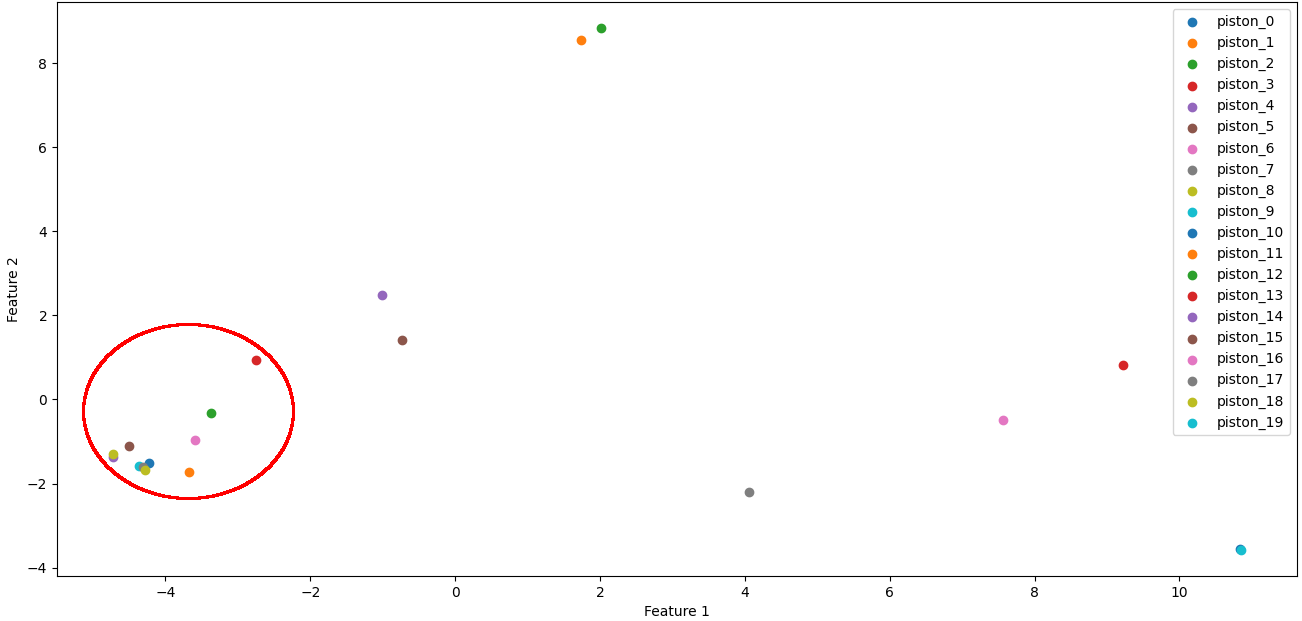
\includegraphics[width=0.45\textwidth]{figures/prahom_pca_analysis.png}
    \caption{PCA of the trained agents' histories in the PBL environment}
    \label{fig:prahom_pca_analysis}
\end{figure}
%
We evaluate the impact of \emph{PRAHOM} on the following criteria: convergence time ratios between PTS, NTS, and FTS for reaching a threshold cumulative reward. Performance stability shows how the trained agents can achieve the goal generally by assessing several environments generated with different parameters. Results are presented in Table~\ref{tab:training_AOMEA_results}.
%
\begin{table}[t!]

    \centering

    \begin{tblr}{colspec={llll},rows={m},measure=vbox,stretch=-1}

        \textbf{Environment} & \textbf{PTS/NTS} & \textbf{PTS/FTS} & \textbf{Perf. stability \\ (avg. / max)} \\

        \hline

        { PPL }
        & { 4.7 }
        & { 1.3 }
        & { 0.9 } \\

        \hline[dashed]

        { PPY }
        & { 6.3 }
        & { 2.2 }
        & { 0.78 } \\

        \hline[dashed]

        { KAZ }
        & { 4.0 }
        & { 1.1 }
        & { 0.42 } \\

        \hline[dashed]

        { CYB }
        & { 12 }
        & { 3.3 }
        & { 0.36 } \\


    \end{tblr}

    \caption{View of the AOMEA approach impact during training}

    \label{tab:training_AOMEA_results}

\end{table}

%
As a general observation, we can notice convergence time is longer for NTS than for PTS which is also longer than for FTS. As expected, the search space is decreasing, hence a shorter convergence time. For instance, we noticed a faster convergence to a sub-optimal solution in the PBL environment by providing organizational specifications as presented in \autoref{fig:prahom_learning_curve}. Although PTS converges faster than NTS to a comparable cumulative reward, NTS may outperform PTS because trained agents' policies are hand-tailored to solve the problem much more finely than the designer's organizational specifications can do. Low-performance stability in the CYB environment indicates the trained agents have difficulty finding general strategies compared to the agents in the other environments.

We also took into account the following criteria after training: roles, links, and global performance. A qualitative analysis is presented in Table~\ref{tab:trained_AOMEA_results}
%
\begin{table}[t!]

    \centering

    \begin{tblr}{colspec={llll},rows={m},measure=vbox,stretch=-1}

        \textbf{Environment} & \textbf{Roles} & \textbf{Links} & \textbf{Global performance} \\

        \hline

        { 1 }
        & {  }
        & {  } \\
        & {  } \\

        \hline[dashed]

        { 2 }
        & {  }
        & {  } \\
        & {  } \\

        \hline[dashed]

        { 3 }
        & {  }
        & {  } \\
        & {  } \\

        \hline[dashed]

        { 4 }
        & {  }
        & {  } \\
        & {  } \\

        \hline[dashed]

        { 5 }
        & {  }
        & {  } \\
        & {  } \\

    \end{tblr}

    \caption{View of the OOMARL approach impact after training}

    \label{tab:trained_OOMARL_results}

\end{table}

%
% //TODO: Moise+ schemes and comparison with expected ones
%
For the PBL environment, we can notice roles being equivalent for agents are expected to act the same. Indeed, trained agents' histories are close hence showing a common emerging role. We generate the PCA presented in \autoref{fig:prahom_pca_analysis} by expressing agents' histories as vectors containing the observation-action couples. We can notice most agents’ histories are in the left bottom zone (circled in red). It shows most pistons seem to act similarly as expected. We observe no organizational specifications except roles have been generated because agents cannot communicate. For the KAZ environment, we can notice two distinct roles: archers tend to move away from zombies, while knights tend to approach them. For the PPY environment, we can observe the output specifications indicate authority links between the leader predator and the simple predators to enable collective strategies for circling prey. Finally, the CYB environment shows communications between blue agents are indeed understood as communication links that enable isolating infiltrated drones or trying to fix and alert recently suspected drones.

\section{Conclusion}

% résumer nos contributions et nos principales conclusions.

% importance d’améliorer l’explicabilité de l’IA dans les systèmes MARL et souligner l’impact potentiel de PRAHOM sur l’avancement du domaine.

% proposer des remarques finales et décrire les orientations des recherches futures afin d’explorer et d’affiner davantage notre algo.

Multi-agent methods rely on the designer's knowledge to design a suitable MAS organization, but do not provide automatic means to determine the relevant organizational mechanisms only from the design requirements and the overall objective.
MARL techniques have been successfully applied to automatically train agents to achieve a given objective without explicit characterization of emerging collective strategies.
The PRAHOM's originality is to enrich a MARL process with an explicit organizational model towards a methodological objective to address these issues. It links the agents' policies (modeled in a Dec-POMDP) with $\mathcal{M}OISE^+$ through the process PRAHOM. Under the simplifying conditions of a group and a single social pattern, PRAHOM makes it possible to partially determine organizational specifications from joint histories and to constrain the training of policies in relation to organizational specifications.
Additionally, we implemented the \emph{PRAHOM PettingZoo} wrapper as a proof of concept to apply PRAHOM.
Finally, we applied our approach in four \emph{PettingZoo} environments to evaluate the impact during and after training. The performances obtained appear to be comparable to those known.

Even if PRAHOM is agnostic with regard to the MARL algorithm, because it uses the history of agents to infer organizational specifications, reconstructing the collective behaviors of agents a posteriori can prove difficult. Indeed, a major perspective to improve PRAHOM is to go further with unsupervised learning techniques in addition to empirical statistical approaches to identify relevant organizational specifications from joint histories. In addition, work from hierarchical learning can contribute to better characterizing emerging strategies during learning.
Ultimately, we also aim to improve the applicability of PRAHOM by developing dedicated interfaces built around PRAHOM making it more accessible to industrial and research contexts.


%%%%%%%%%%%%%%%%%%%%%%%%%%%%%%%%%%%%%%%%%%%%%%%%%%%%%%%%%%%%%%%%%%%%%%%%

%%% Use this environment to include acknowledgements (optional).
%%% This will be omitted in doubleblind mode.

\begin{ack}
    This work was supported by \emph{Thales Land Air Systems} within the framework of the \emph{Cyb'Air} chair and the \emph{AICA IWG}.
\end{ack}

%%%%%%%%%%%%%%%%%%%%%%%%%%%%%%%%%%%%%%%%%%%%%%%%%%%%%%%%%%%%%%%%%%%%%%%%

%%% Use this command to include your bibliography file.

\bibliography{references}

% \newpage

\section*{Annexes}

\subsection*{Action constraining during training implies result joint-policy constraining}
\begin{proofoutline}\label{proof:jpc_to_ac}

    We provide an overview of our approach to constrain the possible policies of trained agents through a simple abstract example. While this example is somewhat artificial, it serves to illustrate the general principle of our approach and gives insights into why it is indeed effective in constraining policies.

    \noindent Let's consider an example with this initial configuration:

    \begin{itemize}
        \item $d=\langle S,A,T,R,\Omega, O, \gamma \rangle \in D$, the Dec-POMDP to solve (i.e maximizing $R$);
        \item $\mathcal{A}, |\mathcal{A}| = n \in \mathbb{N}$, the  $n$ agents involved in the Dec-POMDP;
        \item $s \in \mathbb{R}$, the cumulative reward expectancy to reach;
        \item $\pi_{joint} \in \Pi_{joint}, \allowbreak \pi_{joint} = \{\pi_1..\pi_n\}, \pi_k \in \Pi (k \leq n)$, the joint-policy to update;
        \item $ep_{max}$, the maximum number of episodes;
        \item $step_{max}$, the maximum number of steps per episode;
        \item $u_{marl}: \Pi_{joint} \times H_{joint} \times R_{joint} \rightarrow \Pi_{joint}$, the MARL algorithm that uses the joint-reward and joint-history to update a joint-policy;
    \end{itemize}
    %
    \noindent We assume some organizational specifications are defined, applied to agents, and associated with matching history subsets (at least from a theoretical point view):
    \item $os \in \mathcal{OS}$, the organizational specifications containing: $\mathcal{R}$, the roles that agents may be constrained to; $\mathcal{M}$, the missions that agents may be committed to; $\mathcal{OBL}$, the obligations indicating whether an agent playing a role $\rho \in \mathcal{R}$ is obligated to commit on mission $m \in \mathcal{M}$. In this example, we do not consider permissions; $rh: \mathcal{R} \rightarrow \mathcal{P}(H)$: gives the expected history subset for a role; $mh: \mathcal{M} \rightarrow \mathcal{P}(H)$: gives the expected history subset for a mission; $da: \mathcal{OBL} \rightarrow \mathcal{P}(A)$: gives the agents constrained to a role and obligated to commit on a mission.

    \

    \noindent We suppose there exists a set of joint-policies $S\Pi_{joint} = \{s\pi_{joint,1}.. s\pi_{joint,d}\} \allowbreak (d \in \mathbb{N})$, that enables reaching at least the $s$ cumulative reward expectancy.

    \noindent We suppose there exists a set of joint-policies $O\Pi_{joint} = \{o\pi_{joint,1}.. o\pi_{joint,d'}\} (d' \in \mathbb{N})$ that satisfy the applied organizational specifications, so that an agent playing role $\rho \in \mathcal{R}$ and obligated to commit on mission $m \in \mathcal{M}$ should have its policy $o\pi_{joint,i} \ (i \leq d')$ to generate any matching history $h \in (rh(\rho) \cap mh(m))$.

    \noindent We assume there exists a non-empty set of joint-policies $P\Pi = S\Pi \cap O\Pi \allowbreak = \{p\pi_{joint,1}..p\pi_{joint,q}\}, q \in \mathbb{N}$ that both reach at least the $s$ cumulative reward expectancy and satisfy the organizational specifications $os$.

    \

    Based on these assumptions and initial data, we apply PRAHOM on the first iterations and generalize it to indefinite number of iteration, in order to determine whether it enables building a policy that does belong to $P\Pi$. Although all constraints integration modes are effective in constraining policies, in this example, we chose the $correct\_policy$ mode to apply our algorithm for it offers a clear way to understand the proof outline.
    We consider the first episode. Initially, a constrained policy $\pi_{joint} = \pi_{joint,c}$ built from the initial policy $\pi_{joint,init,0}$ and the observable policy constraint $c\pi_{joint}$.

    At first step, agents have an empty history $h_{joint} = \langle \rangle$, null rewards $rh_{joint} = \langle (0)^n \rangle $. Thus, the initial policies $\pi_{joint,0} \in \Pi_{joint}$ are not updated for now. Receiving the initial observations for each agents $\omega_{joint,0} \in \Omega_{joint}$, agents choose their respective next actions $a_{joint,0}$ using their policies $\allowbreak \pi_{joint,0}$. The observations and actions are stored in history $h_{joint} \allowbreak = \allowbreak \langle \allowbreak (\omega_{joint,0}, \allowbreak a_{joint,0}) \rangle$. Then, the action are applied, hence generating new observations $\omega_{joint,1}$ and rewards $r_{joint,1}$ stored in $rh_{joint}$ for the next step.

    % \

    % At second step, agents have the current history $h_{joint} = \langle (\omega_{joint,0}, a_{joint,0}) \rangle$, and rewards $rh_{joint} = \langle (0)^n, r_{joint,1} \rangle$. Thus, the policies are updated accordingly $\pi_{joint,1} = u_{marl}(\pi_{joint,0},h_{joint},rh_{joint})$. From received observation $\omega_{joint,1}$, agents choose their next actions $a_{joint,1}$ using their policies $\pi_{joint,1}$. The observations and actions are stored in the joint-histories $h_{joint} = \langle (\omega_{joint,0},a_{joint,0}), (\omega_{joint,1},a_{joint,1}) \rangle$. Then, the actions are applied, hence generating new observations $\omega_{joint,2}$ and rewards $r_{joint,2}$ stored in $rh_{joint}$ for the next step.

    Generalizing until the $p < step_{max}$ step, agents have the current history $h_{joint} = \langle (\omega_{joint,0}, \allowbreak a_{joint,0}), (\omega_{joint,1}, a_{joint,1})..(\omega_{joint,p-1}, a_{joint,p-1}) \rangle$, and rewards $rh_{joint} = \langle (0)^n, r_{joint,1}, r_{joint,2}..r_{joint,p} \rangle$. Thus, the policies are updated accordingly $\pi_{joint,p} = u_{marl}(\pi_{joint,p-1},h_{joint},rh_{joint})$. From received observation $\omega_{joint,p}$, agents choose their next actions $a_{joint,p}$ using their policies $\pi_{joint,p}$. The observations and actions are stored in history $h_{joint} \allowbreak = \allowbreak \langle \allowbreak (\omega_{joint,0},a_{joint,0}), \allowbreak (\omega_{joint,1},a_{joint,1}), (\omega_{joint,2},a_{joint,2})..(\omega_{joint,p},a_{joint,p}) \rangle$. Then, the actions are applied, hence generating new observations $\omega_{joint,p+1}$ and rewards $r_{joint,p+1}$ stored in $rh_{joint}$ for the next step.

    \

    When $p = step_{max}$, the episode is finished, we assume the cumulative reward reaches at least $s$. The generated histories are $h_{joint} = \langle (\omega_{joint,0}, \allowbreak a_{joint,0}) .. \allowbreak (\omega_{joint,step_{max}},a_{joint,step_{max}}) \rangle$. Throughout all steps, it is built using the $\pi_{joint,k}, \allowbreak k < step_{max}$ and $\pi_{joint,k} \allowbreak = \allowbreak \{sample(c\pi_{joint}(\omega_{joint})) \allowbreak \ \allowbreak if \allowbreak \ \allowbreak \omega_{joint} \in Dom(c\pi_{joint}) \allowbreak \ \allowbreak else \allowbreak \ \allowbreak \pi_{joint,k}(\omega_{joint,init,k})\}$.
    %
    By definition, $\langle (\omega_{joint,j}, \allowbreak sample(c\pi_{joint}(\omega_{joint,j}))), \allowbreak j < step_{max} \rangle, \allowbreak \omega_{joint,j} \allowbreak \in \Omega_{joint}$, the joint-history generated using the observable constrained policy satisfy the organizational specifications. Thus, the policy represented by $sample(c\pi_{joint}(\omega_{joint,j}))$ belongs to $O\Pi_{joint}$ and possibly $S\Pi_{joint}$.
    %
    By construction, $\langle (\pi_{joint,init,k}(\omega_{joint,k}))_{k < step_{max}} \rangle$, the joint-history generated using the initial policy trained over $k$ steps so that the cumulative reward reach at least $s$. Thus, the policy $\pi_{joint,init,step_{max}}$ belong to $S\Pi_{joint}$.

    Considering several episodes, $s$ is reach for a policy in $\allowbreak S\Pi_{joint,ep_{max},step_{max}}$. Moreover, since a history $h_{joint}$ belongs, at least, to histories generated by a policy in $O\Pi_{joint}$. Thus, $\pi_{joint,ep_{max},step_{max}} \in S\Pi \cap O\Pi, \pi_{joint,ep_{max},step_{max}} \in P\Pi$. So, built policies indeed satisfy organizational specifications while reaching sufficient cumulative reward expectancy.

    \

    As for the other constraint integration modes, we briefly outline the main ideas supporting why it is also effective as well as the $correct\_policy$ mode:
    $\mathbf{correct}$, corrects the action according to an observable policy constraint after the initial policy has chosen it. Without other consideration, it can be modeled by building a constrained policy $\pi_c$ encompassing both the observable policy constraint and the initial policy. Therefore, this goes back to the $correct\_policy$ case;
    $\mathbf{penalize}$, adjust the reward comparing chosen action by the policy and the expected ones according to an observable policy constraint. We assume that the policy can be updated according to rewards so that it asymptotically tends be equal to any constrained policy formed from the current policy and the observable policy constraint. Therefore, it also goes back to the $correct\_policy$ case.

\end{proofoutline}

\end{document}
%%%%%%%%%%%%%%%%%%%%%%%%%%%%%%%%%%%%%%%%%%%%%%%%%%%%%%%%%%%%%%%%%%%%%%
